\documentclass{sigchi}

% Use this command to override the default ACM copyright statement (e.g. for preprints). 
% Consult the conference website for the camera-ready copyright statement.
\toappear{
	Submitted for review.
}

% Arabic page numbers for submission. 
% Remove this line to eliminate page numbers for the camera ready copy
\pagenumbering{arabic}

% Load basic packages
\usepackage{balance}  % to better equalize the last page
\usepackage{graphics} % for EPS, load graphicx instead
\usepackage{times}    % comment if you want LaTeX's default font
%\renewcommand{\ttdefault}{cmtt}
%\usepackage{fontspec}
%\setmainfont{Cardo}
\usepackage{url}      % llt: nicely formatted URLs

% llt: Define a global style for URLs, rather that the default one
\makeatletter
\def\url@leostyle{%
  \@ifundefined{selectfont}{\def\UrlFont{\sf}}{\def\UrlFont{\small\bf\ttfamily}}}
\makeatother
\urlstyle{leo}


% To make various LaTeX processors do the right thing with page size.
\def\pprw{8.5in}
\def\pprh{11in}
\special{papersize=\pprw,\pprh}
\setlength{\paperwidth}{\pprw}
\setlength{\paperheight}{\pprh}
\setlength{\pdfpagewidth}{\pprw}
\setlength{\pdfpageheight}{\pprh}

% Make sure hyperref comes last of your loaded packages, 
% to give it a fighting chance of not being over-written, 
% since its job is to redefine many LaTeX commands.
\usepackage[pdftex]{hyperref}
\hypersetup{
pdftitle={SIGCHI Conference Proceedings Format},
pdfauthor={LaTeX},
pdfkeywords={SIGCHI, proceedings, archival format},
bookmarksnumbered,
pdfstartview={FitH},
colorlinks,
citecolor=black,
filecolor=black,
linkcolor=black,
urlcolor=black,
breaklinks=true,
}

% create a shortcut to typeset table headings
\newcommand\tabhead[1]{\small\textbf{#1}}


% End of preamble. Here it comes the document.
\begin{document}

\title{DeduceIt! Automatically Guiding Students through Derivations in a Massively Open On-line Course}

\numberofauthors{1}
\author{
  \alignauthor Ethan Fast, Colleen Lee, Michael Bernstein, Daphne Koller, Alex Aiken\\
    \affaddr{Stanford University}\\
    \email{\{ethan.fast, clee0, msb, koller, aiken\}@cs.stanford.edu}\\
}

\maketitle

\begin{abstract}
This paper presents DeduceIt, a derivation checking system for massively open on-line courses. DeduceIt is a general system for creating and grading student assignments---it guides students through exercises which can be defined by instructors across arbitrary formal domains---but unlike other interactive theorem provers, it presents a web-based interface accessible to non-expert users, and it can be used by instructors and students without prior training. DeduceIt also introduces the idea of a \textit{proof cache}, a novel data structure which leverages a crowd of students to decrease the cost of checking derivations and providing real-time, constructive feedback. We describe our experience using DeduceIt and evaluate the system with data collected from thousands of students in an on-line class.
\end{abstract}

\keywords{
	\textcolor{red}{What keywords to use?}
}

\category{H.5.m.}{Information Interfaces and Presentation (e.g. HCI)}{Miscellaneous}

% See: \url{http://www.acm.org/about/class/1998/}
% \textcolor{red}{Mandatory}

\terms{
	Human Factors; Design; Measurement. 
}

% \url{http://www.sheridanprinting.com/sigchi/generalterms.htm}.
% \textcolor{red}{Optional section to be included in your final version.}

\section{Introduction}
As instructors begin to teach hundreds of thousands of students in on-line classrooms, it becomes increasingly difficult for them to grade complex assignments and provide students with personal feedback. Here, the rise of massively open on-line courses (MOOCs) presents a departure from the standard educational model: TAs are not designed to scale. 

% In some ways this is not a problem. Often when one student is stuck on an assignment, or fails to understand a lecture, another more knowledgable student will step in to help. Our experience instructing an on-line Compilers class suggests that communities form dynamically around on-line courses, providing students with an emergent network of peer support.

% However, student communities cannot entirely replace the roles Professors and TAs. Even the most capable of students will tend to lack the domain knowledge of the instructor, and when feedback occurs---usually on some kind of forum--

When the size of an on-line course increases, the attention of its instructors and TAs necessarily becomes more scarce. They are unable to provide large numbers of students---to date the largest MOOC has enrolled more than 180,000 \cite{enroll}---with feedback on their assignments; much less to present it in real-time. In particular, grading becomes intractable unless it is automated. But automation is often hard to achieve, particularly in complex domains where students may construct correct solutions in many different ways. \cite{automated-scoring-design, automated-grading}

These constraints are important limitations to the MOOC model. Students tend to learn better when subject to tight and personal feedback loops \cite{personalized-feedback} and many subjects, when taken in a traditional class setting, grade students on proofs or derivations where there are many ways to describe a correct answer.

MOOC platforms have attempted to automate away some of these issues, but providing thousands of students with \textit{constructive} and \textit{real-time} feedback has remained an unsolved problem. \cite{derivation-scoring} Coursera and Udacity give instructors out-of-the-box tools to build assignments and quizzes with automated grading features, but these tools lack flexibility: evaluation is constrained to discrete, instructor-specified solutions and offers students a limited feedback loop (e.g. ``correct," or ``incorrect"). \cite{fixme} For technical, mathematical, or scientific domains where assignment solutions are often \textit{derivations}---many-staged and prone to individual variation---this limitation is particularly problematic. \cite{derivation-scoring} And other related research suggests that as a system departs further from a traditional ``pen and paper" interface, a greater cognitive load is placed upon the student. \cite{interface-learning-load}

To address these limitations we present:
%(e.g. in our Compilers course we use it to assign problems in type checking, regular expressions, finite automata, and many other topics; its generality allows its use in most formal systems).
\begin{itemize}
\item The \textit{DeduceIt} system: A web-based framework in which it is possible to specify a general class of derivation exercises, yet which remains accessible non-expert users. DeduceIt provides students with constructive and real-time feedback.
\item The idea of a \textit{proof cache}: A novel data structure which records the history of every attempted derivation, reusing computations from previously derived steps to provide predictable performance under heavy load and enable real-time feedback on student progress. We show this cache can increase system efficiency by several orders of magnitude.
\item An \textit{empirical evaluation} of DeduceIt: A report on the data we have collected from a massive on-line class with thousands of students doing dozens of exercises.
\end{itemize}

The rest of this paper is organized as follows: We begin with related work and a motivating example, then present DeduceIt's interface and capabilities. Next, we describe the underlying architecture of the system and provide an empirical evaluation, using data collected from students in an on-line class. We close with reflections, conclusions, and future work.

\section{Related Work}
At its core, DeduceIt is an interactive proof solving system, and there exists quite a bit of related work on this subject. Many existing tools already provide users with rich and automated feedback as a form of proof assistance \cite{coq,maude,isabelle, isabelle1,lisp-logic}, but these tools are designed for experts and are generally unsuited to the MOOC audience. For instance, tools like \textit{coq} and \textit{isabelle} allow users to explore complex problem domains (e.g. isabelle has been used to encode ideas as nuanced as Godel's Incompleteness Theorem), but their interfaces are not designed to be accessible to lay students or---depending on the course in question---even to a typical instructor. 

Some prior work has looked specifically at applying automated theorem provers in an educational context. \cite{suppes, suppes-prover} In fact, DeduceIt draws a great deal on the insights of researches like \textit{Suppes}, and the idea of using theorem provers to enable education has engendered much discussion among researchers. \cite{automated-grading, automated-scoring-design} However, even systems designed to address educational use have tended toward complicated interfaces, typically involving unstructured interactions with a terminal-like environment. Moreover, no such system has been deployed at web scale to serve thousands of students. [Fixme: more examples of these systems, if any?]

There exists other more domain specific work in automatic feedback and grading systems. Simple forms of automatic grading have been studied in both physical and on-line classrooms [fixme: citation]. These systems tend to restrict an assignment's answer domain with assumptions like multiple choice answers, concrete-valued answers (e.g. answers that match against a string or numerical value), or a set of test cases to evaluate a programming assignment. While restricting the answer domain can work well for certain subjects or applications, in general it does not grant an instructor sufficient means to evaluate more creative or complex assignments. There exist various exceptions here as well: for instance, automated grading and plagiarism detection systems have long evaluated student program code---where solutions may be unstructured and creative---in computer science departments \cite{grade-programs, moss}, and also commercially. We are concerned here with a different kind of system.

Finally, crowdsourcing research has enabled new forms of problem-solving and evaluation. For instance, peer consistency evaluation can be used to effectively judge the accuracy---and grade---of a student's answer, even in the absence of a ground truth \cite{peer-consistency}; crowd-based peer assessment has been successfully applied to grade student assignments \cite{peer-assessment}; and crowds have been used to detect and generate various canonical features of a language, like code snippets for use in an IDE. \cite{crowd-snippets}. While DeduceIt's proof cache draws inspiration from crowd research---the system leverages the results of one student to help another---humans are never directly involved in assignment evaluation. We hope to further involve the crowd in DeduceIt's computations as a subject of future work.

\begin{figure}[!h]
\centering
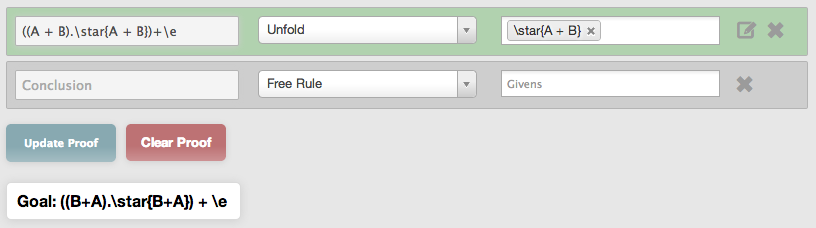
\includegraphics[width=1\columnwidth]{emptyline}
\caption{A derivation prompts the user to enter another step.}
\label{fig:emptyline}
\end{figure}


\begin{figure}[!h]
\centering
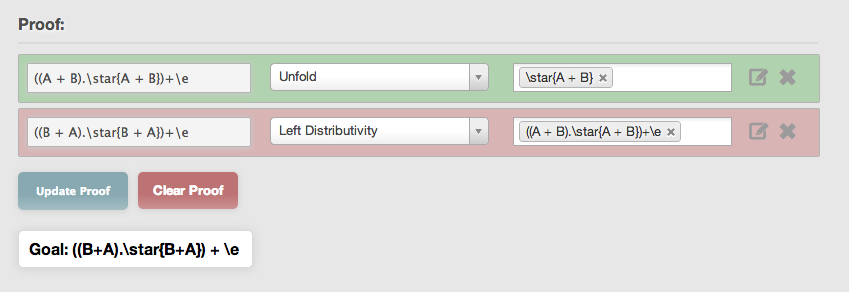
\includegraphics[width=1\columnwidth]{regexproof}
\caption{A derivation with correct and incorrect steps.}
\label{fig:regexproof}
\end{figure}

\begin{figure}[!h]
\centering
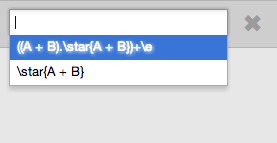
\includegraphics[width=0.7\columnwidth]{selectassumptions}
\caption{Selecting assumptions in a derivation. These include the givens and any expressions proven earlier in the derivation.}
\label{fig:selectassumptions}
\end{figure}

\begin{figure}[!h]
\centering
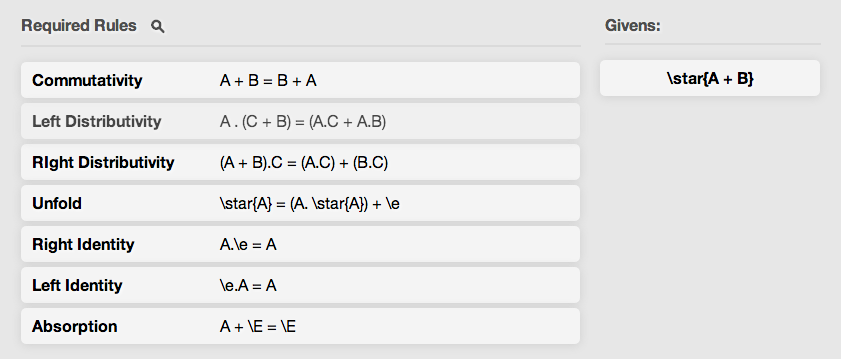
\includegraphics[width=1\columnwidth]{rules}
\caption{The set of rules available to a user.}
\label{fig:rules}
\end{figure}

\section{Motivating Example}

To better motivate how DeduceIt works and what problems it solves, we begin with an example assignment from the perspective of a MOOC student in Coursera's Compilers class. This student has recently finished her first week in the course, where she has learned among other things about the properties of regular expressions.

In this particular assignment we ask her to show equality between two regular expressions. Assuming $+$, $*$, and $.$ as union, kleen closure, and concatenation, she must prove:
$$(A+B)* \equiv ((B+A).(B+A)*)+\epsilon$$
More concretely, the assignment asks our student to derive a particular expression. DeduceIt labels this the \textit{goal}: 
$$((B+A).(B+A)*)+\epsilon$$ 
To show the goal expression, our student must start from certain other expression(s). DeduceIt calls these the \textit{givens}, and here they consist of the single starting expression: 
$$(A+B)*$$
Our student also sees a description of the assignment and---perhaps most importantly---the available \textit{rules} she may apply on the given expressions (or in some cases, sub-expressions of these givens) in order to derive the final, goal expression. In this assignment these rules specify several equality preserving transformations of regular expressions: Commutativity, Distributivity, Right Distributivity, Unfold, Identity, Left Identity, and Absorption. However, rules may not always preserve equality in general.

To complete a step in the derivation, our student may apply a rule to one or more given expressions, producing a new \textit{conclusion}. As the derivation expands, the conclusion of each previous step is added to the set of givens. DeduceIt can provide several different kinds of feedback on each step, depending on the state of the derivation. Next, we will walk through a few such steps.

\subsection{Completing a Derivation}
As she reads over the assignment, our student realizes she has only been given one expression from which to start her derivation: $(A+B)∗$. She reasons this must go in the givens input field on the first step. (In fact, this is the only expression DeduceIt allows her to enter in that field). Now she has two input fields left. One asks for a rule; the other a conclusion. To come up with a conclusion, she must decide which rule to apply, and where to apply it. She supposes ``Unfold" looks promising and tries it on the full starting expression, computing:
$$((A + B).(A + B)*)+\epsilon$$
This expression looks pretty close to her goal, so she enters it in the conclusion input field. After selecting ``Unfold" as her rule, she tells DeduceIt to update her derivation. There is a brief computation, then the derivation returns with her previous step highlighted in green: it was successful. A new step lies below her previous entry---this one is empty---querying her for the next line of the derivation.

Our student now considers her previous conclusion: since it is nearly identical to the goal, she wants to use it for her next step. If she can transform its two sub-expressions $A+B$ to $B+A$, then she will have proven the goal and completed the assignment. While she is pretty sure one property of regular expressions does allow for this kind of transformation, she can't remember what it is called. So she looks through the assignment rules and sees it: Commutativity! Regular expressions are commutative under union.

Mentally, she applies Commutativity to each of the two $A+B$ sub-expressions, then enters her result in the conclusion input box on the next line of the derivation. This conclusion is identical to the goal expression: 
$$((B+A).(B+A)*)+\epsilon$$
She selects ``Commutativity" from the rule input box, chooses the conclusion from her previous step $((B+A).(B+A)*)+\epsilon$ as her new given, and tells DeduceIt to  update her proof. DeduceIt checks her derivation, infers through proof search that she means to apply Commutativity twice---on the two appropriate sub-expressions---and responds that the derivation is correct: she has completed this assignment.


\section{How DeduceIt Works}

We begin this section with background information about term rewriting systems, then we present an overview of DeduceIt's two primary interfaces: the instructor view and the student view.

\subsection{Term Rewriting Systems}

DeduceIt uses a term rewriting system to verify student derivations. In general, a rewriting system consists of a set of objects and relations which define transformations on those objects; each transformation is called a rewrite rule. A \textit{term} rewriting system is a rewriting system which operates on expressions with nested sub-expressions. \cite{rewriting-logic, isabelle}

Term rewrite rules define transformations which occur between terms. These rules have a left side, which must match a term for the rule to be applied, and a right side, which defines the new expression produced by the rule. Variables may appear in the rule (declared in the system with $\$$ notation) which bind to the term or its subexpressions. For example, in a language which supports integers, symbols, and the binary operators $+$, $-$, and $=$ (this happens to be a subset of the default DeduceIt language), one such rule might be: $(\$x+\$y=\$z) \rightarrow (\$x=\$z-\$y)$. The system can apply this rule to the expression $2+1=3$ to produce $2=3-1$.

While DeduceIt's derivation checker operates primarily as a term rewriting system, it differs from a standard system in several respects. First, DeduceIt supports an assumption of equality in certain rewrites, where specified by an instructor. Rewrite rules which assume equality (declared with $:=$ instead of $\rightarrow$) can be applied recursively upon term subexpressions; the entire term need not match the rule, but only a subexpression of that term. This makes DeduceIt more efficient at verifying certain common derivations. Second, DeduceIt supports the dynamic evaluation of basic mathematical expressions. \cite{dynamic-rules} For instance, if DeduceIt is provided with a set of rules which govern basic algebra and the expression $x=3-1$, it can derive $x=2$ by using the dynamic rule $\$x-\$y := eval(\$x-\$y)$. This rewrite is also an example of a rule which assumes equality.

%Fixme: talkabout conditional rules

\begin{figure}[!h]
\centering
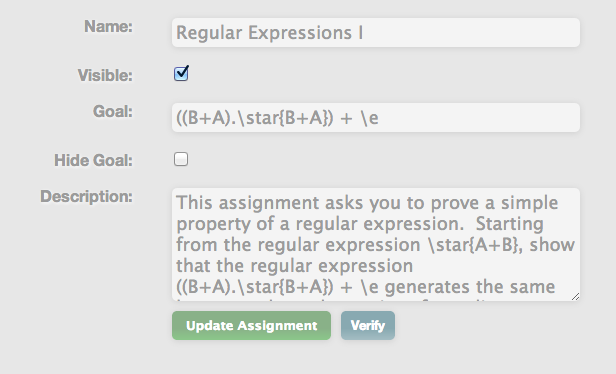
\includegraphics[width=1\columnwidth]{assign_meta}
\caption{Basic data associated with an assignment.}
\label{fig:assign_meta}
\end{figure}

\begin{figure}[!h]
\centering
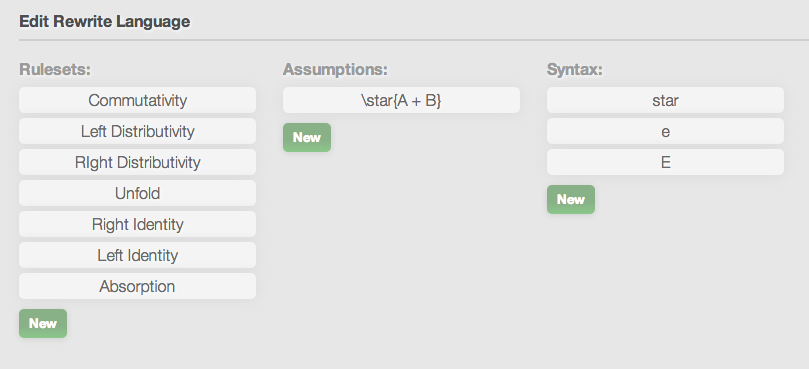
\includegraphics[width=1\columnwidth]{rewrite_language}
\caption{Instructors must specify a rewrite language for each assignment.}
\label{fig:rewrite_language}
\end{figure}

\begin{figure}[!h]
\centering
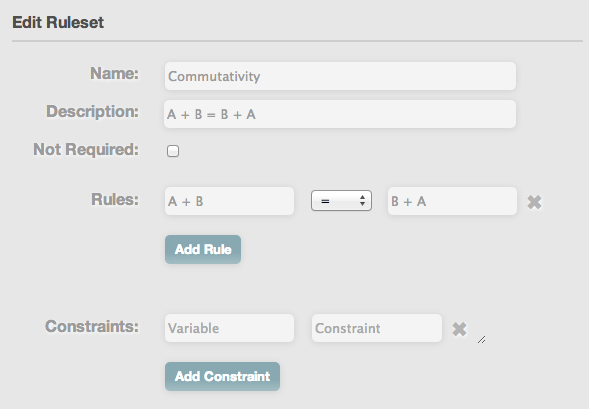
\includegraphics[width=1\columnwidth]{editruleset}
\caption{Editing a ruleset on the instructor interface.}
\label{fig:editruleset}
\end{figure}

\begin{figure}[!h]
\centering
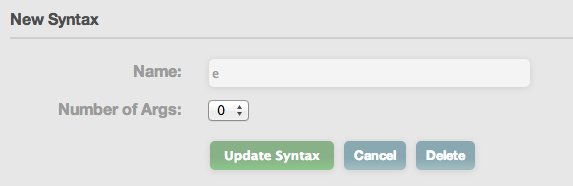
\includegraphics[width=1\columnwidth]{syntax}
\caption{Adding new syntax on the instructor interface.}
\label{fig:syntax}
\end{figure}

\subsection{The instructor view}

The assignment construction page is the most complex portion of DeduceIt's interface. To create an assignment, an instructor must specify four things: 
  \begin{enumerate}
  \item A rewrite language: DeduceIt provides every assignment with a default rewrite language composed of variables, symbols, integers, and several common unary and binary operators. In many assignment domains this will be sufficient, but an instructor may optionally augment the language with extra syntax for functions and constants. 
  \item The Rulesets: These are named sets of rewrite rules which a student may apply while working through an assignment's derivation. One ruleset corresponds to many underlying rewrite rules. This is necessary because an instructor may want to refer to several distinct rules by the same name (e.g. $1*X \rightarrow X$ and $X*1 \rightarrow X$ are two distinct rewrite rules which both describe the multiplicative identity.)
  \item The given expression(s): A set of expressions which serve as the starting point of a derivation.
  \item The goal expression: The desired result of a derivation.
  \end{enumerate}

A student works through an assignment by starting from the given expressions and applying valid transformations until she has reached the goal expression.

\subsubsection{The Language}

DeduceIt's default language should be familiar to anyone who has used an advanced calculator. It ships with the unary operators $\char`\~$ and $-$, and the binary operators $.$, $\&$, $|$, $,$, $*$, $\backslash$, $+$, $-$, $=$, $\neq$, $\leq$, $\geq$, $<$, $>$, $:=$, and $\rightarrow$ which we list in order of precedence. DeduceIt also supports variables (these may only be used when defining rewrite rules), symbols, and integers. For example, here are three legal expressions in the default rewrite language are: 
$$\$p,(\$p=>\$q)\rightarrow{}\$q$$ 
$$a.b.b.a$$
$$x+2=y$$ 
Note that with three exceptions (the notation specific to rewrites: $:=$, $\rightarrow$, and $\$$) the operators used in these expressions have no meaning without an accompanying set of rules; they simply determine the parsing of an expression.

Instructors may add two kinds of syntax to DeduceIt's standard rewrite language: constants and variable argument functions. This is convenient in many domains, where familiarly named functions and constants enhance the readability of an assignment. For these custom functions and constants DeduceIt adopts a notation inspired by latex. Constants appear in the language as a symbol value preceded by a backslash, e.g $\backslash{}e$. Functions look much the same, except they have arguments which they accept in brackets, e.g. $\backslash{}sin\{x\}$. Figure \ref{fig:syntax} shows DeduceIt's custom syntax creation view.

\subsubsection{Rulesets}

Rulesets are the most complicated part of an assignment. They define the sets of valid transformations which a student may use in a derivation. Each ruleset has a name, a student-facing description, a set of rewrite rules, and an optional set of constraints. The name and description of a ruleset are all a student sees when using DeduceIt, and these fields  make an assignment more accessible; students do not need to understand rewrite rules to use the system.

Each rewrite rule in a ruleset is either a strict rewrite rule or an equality. To apply a strict rewrite rule, its left side must match exactly on an expression, wheres an equality may be applied to an expression or any of its subexpressions. Take as an example the expression $1+y*y=5$ and the strict rewrite rule $\$x*\$x \rightarrow \$x^2$; here the rewrite rule cannot be applied, since its left side doesn't bind with the entire expression. However, a similar rewrite rule which has been defined with an assumption of equality, $\$x*\$x := \$x^2$, will bind on $y*y$ and produce the transformation $1+y^2=5$. In this way equalities are more powerful than strict rewrite rules, and for many assignments a single equality can take the place of many strict rules. This eases the burden on an instructor and usually speeds up proof search; the more rules an assignment has, the slower search tends to be.

Various constraints may be defined on the variable terms used in the ruleset. They operate in a manner similar to conditional rewrite rules, but are somewhat less general; we use only containment---whether or not a variable contains certain other terms---as a condition on ruleset application.

A ruleset may also be either ``required" or ``free." While a required ruleset must be named explicitly when a student uses it in a derivation, a ``free" ruleset may be elided. Behind the scenes, DeduceIt will attempt to fill in such ``free" steps automatically through proof search. This is useful when a student must use trivial transformations which are necessary to the derivation but unimportant to the assignment. For example, a student may want to rearrange terms in a mathematical expression as part of some broader rule application. DeduceIt's ``free" rules allow the student to skip over these steps.  

In figure \ref{fig:editruleset} we show DeduceIt's Ruleset creation view.

\subsubsection{Sharing Rewrite Languages}

Some rewrite languages are common enough that it makes sense to share them among different assignments: for instance, many assignments might use the languages defined for basic algebraic manipulation, predicate logic, or the expansion of regular expressions. DeduceIt allows instructors to reuse a rewrite language across assignments.

\begin{figure}[!h]
\centering
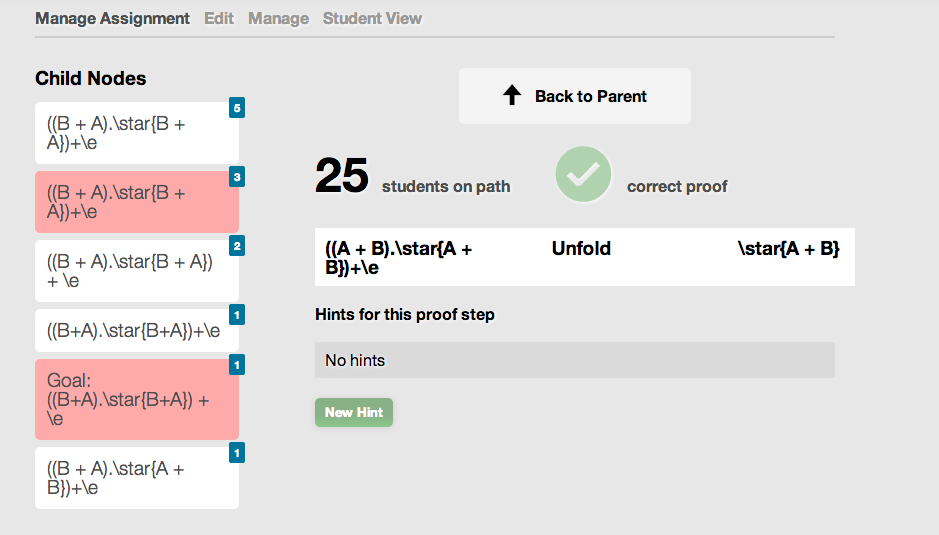
\includegraphics[width=1\columnwidth]{nodeannote}
\caption{Annotating a node on the proof tree.}
\label{fig:nodeannote}
\end{figure}

\subsubsection{The Assignment Proof Tree}

For each assignment, an instructor has real-time access to its proof tree. This tree tracks the history of all derivations associated with the assignment. These derivations share a common root node, and each step in a derivation maps to one of its children, the immediate parent of which is either the root node itself or else a node associated with the previously derived step. Every node keeps track of derivation state information and a count of how many students have traversed it. An instructor may annotate any node in the tree with hints, and these will be visible to a student if she enters upon that path in her own derivation. An instructor may also use this tree to override the behavior of the underlying derivation checker, e.g. forcibly label a given derivation step valid. This can be useful for steps which make use of particularly long chains of free rules which can't be discovered and verified by proof search.


\subsection{The student view}

An assignment's student view presents the information we have already encountered on the instructor interface. At the top of the page a title, goal, and description broadly introduce the exercise at hand. Below these are the given expressions---a student uses one or more of these to start the derivation---and some number of rulesets divided into two types: required and free. Rulesets may be (and usually are) composed of many separate rewrite rules, but an assignment presents them as single, discrete entities; students need not be familiar with rewriting systems to use DeduceIt. In fact, the term `rewrite' cannot be found anywhere on the student view, and these rulesets are themselves labeled on the page simply as `rules'. This might create a leaky abstraction if rulesets are not carefully specified (i.e. the instructor description does not exactly match the behavior specified by the underlying rewrites), but most students are not familiar with rewrite rules, and we have discovered that a small sacrifice of precision in the rules positively impacts usability, as reported by several students.

\subsubsection{Interacting with a Derivation}

Each assignment page contains an interactive derivation. Before a student has made progress in an assignment this derivation consists of only three empty input fields which are labeled: conclusion, rule, and givens. To more forward in a derivation, a student must derive a conclusion by applying the selected rule on the selected givens(s). 

This derivation interface constrains students in several respects. First, students may select only expressions which they have already derived (or which are members of the set of starting givens) from the givens input field. Likewise, students may only select rules which are associated with the current assignment from the rules input field. These constrains eliminate the possibility of many simple mistakes, like mistypings, which we found surprisingly common in an earlier prototype of the system. The conclusion input field is unconstrained, however, and students can type into it any kind of expression they wish.

To verify the current state of a derivation, students must click on the button ``Update Proof." DeduceIt will respond with one of several kinds of feedback: if the derivation is so far valid, all its steps will turn green; if the system cannot parse the conclusion of some step in the derivation, that step will turn yellow; or if the system can parse but not prove the conclusion of some step in the derivation, that step will turn red. Each valid step preceding an invalid step will remain green, and if an invalid step has any hint annotations on the assignment Proof Tree, hints appear adjacent to that step. Hints take the form of a styled question mark, which expands into text on mouseover. Finally, if the conclusion of the latest step is equivalent to the goal expression, DeduceIt signals the assignment is finished with a large checkmark and does not prompt a new step in the derivation.

\subsection{Extensions to the Derivation Interface}

We experimented with several other forms of derivation feedback which we have not yet deployed for our on-line class.

\subsubsection{Surfacing the Proof Path}

DeduceIt maintains aggregate data about every derivation, so the system knows when students are proceeding down well-traveled paths in a derivation, or down correct but---so far---more lengthy paths, or down paths which have not yet led to the goal. One version of DeduceIt surfaces this information with a status indicator, a colored circle of green, yellow, or orange at the top of the derivation, indicating whether students are on a common path, an uncommon but successful path, or an as yet unsuccessful path. 

From anecdotal feedback, it seems students find this indicator helpful, and in theory DeduceIt could provide students even finer grain information: the exact number of other successful or unsuccessful students who have worked to the current state of their derivation; or detection of the exact step in their derivation where they left the well-traveled path. It is also possible to further process the Proof Tree. By collapsing some nodes which are syntactically different but semantically equivalent (e.g. the expressions $(1+2)+3$ and $1+(2+3)$ in a calculus assignment) DeduceIt could construct a more meaningful notion of a derivation path.

\subsubsection{Providing Automatic Hints}

DeduceIt allows instructors to set up hints for any derivation step by annotating an assignment's proof tree. However, we built another version of DeduceIt that constructs these hints automatically using proof search. In this second implementation, DeduceIt holds the rule and assumption fields constant and searches for alternative valid conclusions. 

For instance, suppose a student enters $x=3+1$, \textit{Balance Equation}, and $x+1=3$ in the respective fields for conclusion, rule, and assumptions. This is an incorrect step, so DeduceIt will highlight it in red. And in the standard version of DeduceIt, if an instructor has not annotated this step on the proof tree, this is all the system will do. The student will not be given any further direction; she knows only the step is wrong. However, the hint-generating DeduceIt is able to give her more specific feedback, e.g. ``Your conclusion is incorrect." In this example proof search finds a viable alternative conclusion, $x=3-1$, which matches the rule and assumption the student entered, so DeduceIt knows it is possible to apply the selected rule upon the selected assumptions.

Other hint-generating systems might hold constant different parts of the derivation (e.g. searching for rules and assumptions to match a given conclusion), or leverage the Proof Tree to provide students with hints particular to common derivation paths. It is important to us that the system provide useful hints without giving away too much information: a tricky balance to achieve in an automated system. Hint generation is the subject of ongoing work.

\section{The Internals of DeduceIt}


DeduceIt is a system formed of three distinct components: a frontend interface, a backend theorem prover, and a database. The frontend manages all user interactions (for both students and instructors) as described in the previous section, the backend theorem prover exposes an on-line API which the frontend calls---when necessary---to check student derivations, and the database stores all the data associated with users and assignments, including the Proof Cache.

We built these components using several technologies and cloud providers. The frontend is a Ruby on Rails web application deployed on Heroku, the backend is a Haskell application also deployed on Heroku, and the database is a MongoDB installation running on MongoHQ. Each of these components can be scaled to serve arbitrary numbers of students.

\subsection{The Theorem Prover}

To verify student derivations, DeduceIt applies proof search over a term rewriting system. Its system differs from a standard rewriting system in that it supports rulesets (i.e. named groups of rewrite rules), equalities, dynamic evaluation for some term expressions, and containment conditions on the application of certain rewrites. We discussed each of these features in the previous section. 

DeduceIt's theorem prover also includes a parser which the system constructs dynamically, per API call. This allows instructors to define custom assignment syntax. DeduceIt uses the parser to deconstruct an API call into expression terms of the rewrite language, before it passes these terms to the prover.

\subsubsection{The Theorem Prover API}

The DeduceIt prover is wrapped in web server which can be queried via API on the following POST parameters: \textit{rulesets}, \textit{assumptions}, \textit{syntax}, and \textit{conclusion}. To every query the prover will respond with either ``proven", ``unproven'', or ``syntax error.'' The frontend uses this API to assess the validity of each step in a derivation.

The API parameters function much as their names suggest. The \textit{syntax} parameter defines any new syntax on the default rewrite language. The rest of the parameters are used for proof search: DeduceIt tries to prove the provided \textit{conclusion} expression using the set of rewrite rules defined in \textit{rulesets} on the starting expressions in \textit{assumptions} (that is, assuming all these parameters parse). 

Although in the previous section we mentioned a student can select only one ruleset for each step of a derivation, it is usually necessary to pass the backend prover more than one. This is necessary because the prover requires not only the ruleset selected on the given step, but also any other rulesets which are declared ``free." Free rulesets are always allowed for any step of the derivation; in general they tend to be common or trivial transformations, orthogonal to the didactic goals of an assignment. 

In [fixme] we show an example API query.

\subsubsection{Proof Search}

In DeduceIt, proof search works by applying rewrite rules iteratively upon a group of expressions to generate new expressions. In general, a search may be considered either \textit{forward}, starting from the known expressions and working toward the desired expressions, or \textit{backward}, starting from the desired expressions and working toward the known expressions with an inverted set of rules. DeduceIt supports both kinds of search. 

For example, suppose we give DeduceIt the assumption $a$, the rewrite rule $a \rightarrow a.a$, and the conclusion $a.a.a$. The system may conduct a forward search: start from $a$ and apply the rule twice, first producing $a.a$ and then $a.a.a$. Or it may search backward: construct a new rule $a.a \rightarrow a$ (the inverse of the old rule) and start from $a.a.a$, and then apply this new rule twice to produce $a.a$ and then $a$. Either method leads the system to declare the step valid.

In practice, DeduceIt conducts one round of forward search and one round of backward search; the two rounds of search then meet in the middle, i.e. they check for terms generated in common. We introduce backward search to ensure DeduceIt will correctly check rewrite languages which allow the introduction of new symbols, e.g. predicate logic and the rule $\$a \rightarrow \$a \vee \$b$ (note here that $\$b$ is a variable in the rewrite rule which binds to \textit{any expression}, so forward search cannot enumerate every possible value of $\$b$). Moreover, the meet in the middle approach tends to be more effective than two rounds of only forward or backward search. 

We find the system is limited to two rounds of search under reasonable time constraints: an upper bound of 4 seconds, for students interacting with a web application. At each iteration of search DeduceIt applies the set of available rewrite rules---defined by the collection of rulesets---non-deterministically and exhaustively. 

\subsection{The Proof Cache}

The proof cache is a data structure DeduceIt uses to track all responses the frontend application receives from the prover. This cache is composed of many proof trees, one for each assignment, and together these proof trees track the aggregate history of every attempted derivation (as we discussed in the previous section). Proof trees are useful enough for managing assignments---through them an instructor can annotate derivation steps and override the default behavior of the prover---but they can also, by acting as a cache, potentially improve the overall performance of the system. To check a new derivation step using the proof cache, DeduceIt walks down the proof tree associated with that derivation's assignment: if the new step already exists in the tree, then the system doesn't need to query the prover; it simply returns the stored result.

We formed two hypotheses about the proof cache:
\begin{enumerate}
  \item Students tend to complete their derivations in similar ways; that is, they follow similar paths through an assignment's proof tree.
  \item It is more efficient to reuse the intermediate results of one student's derivation to check the validity of another student's derivation, when compared to checking every derivation step with the prover. 
\end{enumerate}  
  The second hypothesis seemed particularly likely to us since the cost of a checking a step with the prover is much higher than the cost of looking up a result in the cache. An average prover API query takes $4000ms$, whereas a typical cache lookup takes only $900ms$ seconds. We evaluate the performance impact of the proof cache more fully in the next section.

\section{Evaluation}

To better evaluate DeduceIt's usefulness, we deployed it in the winter offering of Coursera's \textit{Compilers} class, where we assigned each student several DeduceIt problems for every week of the course. Out of the 7625 students who enrolled, 1788 of them participated actively, and 1000 (fixme) of these students completed at least one DeduceIt assignment.

In this section we analyze several aspects of the DeduceIt system. We begin with a broad measure of system performance, and then for ten DeduceIt assignments we analyze the distribution of students' time spent on derivations, the success rate of students, the average number of student errors, and the performance impact of the DeduceIt's proof cache. Finally, we take a closer look at three assignments, to provide an example of the new kinds of analyses that DeduceIt enables.

\subsection{System Performance}

In the first experiment, we measure the relation between system latency and load. Since a MOOC will typically enroll thousands of students, it is important that DeduceIt maintain responsiveness when visited concurrently by many users. 

Our analytics show DeduceIt receives one incoming request per minute on average. However, at peak load---usually associated with an assignment deadline---the application may receive up to $X$ incoming requests per minute. Since DeduceIt runs on a cloud provider, we can add necessary resources on demand to handle this additional traffic. 

Over the length of the course, DeduceIt's average latency was $900ms$. At times of peak load, this latency was $1100ms$. 

\begin{figure}[!h]
\centering
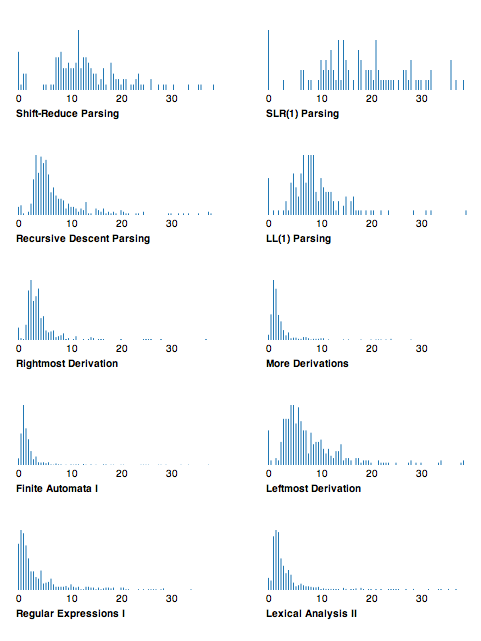
\includegraphics[width=1\columnwidth]{distributions}
\caption{We construct normalized histograms to show the student time distributions for each assignment. The x-axis measures time in minutes.}
\label{fig:distributions}
\end{figure}

\begin{table}[!h]
  \begin{tabular}{|c|c||c|c|c|}
    \hline
    \tabhead{Assignment Name} & \tabhead{Success} & \tabhead{Valid} & \tabhead{Syntax} & \tabhead{Semantic} \\
    \hline
    Regular Expressions I & 96 & 55 & 11 & 34 \\
    \hline
    Lexical Analysis II & 97 & 63 & 6 & 30 \\
    \hline
    Finite Automata I & 98 & 73 & 3 & 23 \\
    \hline
    Leftmost Derivation & 95 & 56 & 6 & 38 \\
    \hline
    Rightmost Derivation & 98 & 81  & 1 & 17 \\
    \hline
    More Derivations & 99 & 81 & 1 & 18 \\
    \hline
    Recursive Descent Parsing & 96 & 69 & 1 & 29 \\
    \hline
    LL(1) Parsing & 99 & 83 & 1 & 15 \\
    \hline
    Shift-Reduce Parsing & 94 & 85 & 2 & 12 \\
    \hline
    SLR(1) Parsing & 93 & 60 & 2 & 36 \\
    \hline
  \end{tabular}
  \caption{We measure student success rates for each assignment and the corresponding student error rates, broken down into syntax errors and semantic errors.}
  \label{tab:table1}
\end{table}

\subsection{Student Time Distributions}

In the second experiment, we analyzed the amount of time students spent on each derivation. Our results are displayed in figure \ref{fig:distributions}. These time distributions are approximately normal and centered upon a fixed time value which tracks loosely with an assignment's difficulty. For example, in the Rightmost Derivation assignment students are clustered around $4$ minutes, and in the Shift-Reduce Parsing assignment they are clustered around $10$ minutes; the Rightmost Derivation assignment was generally considered easier by students than the Shift-Reduce Parsing assignment. This relation also holds true among the remainder of the assignments.

As instructors, we were heartened by the speed at which most students completed even the harder assignments like Shift-Reduce parsing. We were also pleasantly surprised by student success rates, as we will see in the next section.

\subsection{Student Success Rates}

In the third experiment, we examined how the success rates of students vary across assignments. Our results are displayed in table \ref{tab:table1}. Success rates are uniformly high across assignments, ranging from $94\%$ to $98\%$, and these rates also track reported assignment difficulty in a manner consistent with time distributions.

We were also curious whether student success rates are correlated with other assignment features. To this end, we formed several hypotheses. First, we predict that student success is more likely when the length of the shortest viable derivation is smaller. Second, we predict the same when an assignment is less complex (e.g. there are fewer rules or assumptions provided in an assignment). We tested several of these hypotheses, as we show in figure \ref{fixme}.

[Fixme: actually test these? What hypotheses do we want to test, if any?]

\subsection{Student Error Rates}

In the fourth experiment, we look at student error rates. Error rates among derivation steps for all the DeduceIt assignments are substantial, despite the high overall assignment success rates reported in table \ref{tab:table1}. We expected this result; students will always get some things wrong, and learning rarely takes place without error \cite{fixme}. However, ideally we would like to distinguish between two classes of error: errors which stem from a misunderstanding of course material, and errors which stem from misunderstandings associated with the DeduceIt interface.

To approximate the impact of these two classes of error, we divide student mistakes into two categories: syntax errors, and semantic errors. Syntax errors arise from entering an expression which DeduceIt cannot parse, whereas semantic errors arise from parseable derivation steps which cannot be proven. While semantic errors are certain to contain faulty logic, this is not obviously true for syntax errors: a student might have intended to write a correct step and simply failed to use the system properly. We use the rates of student syntax errors as a proxy for measuring rates of student confusion with the DeduceIt system.

Across all assignments syntax errors are low, never exceeding $11\%$. Notably, the highest rate of syntax errors occurred in the first class assignment, Regular Expression I, despite the fact that students generally considered this assignment the easiest. The syntax error rates of subsequent assignments never exceeded $6\%$, although these later assignments were much more difficult. This suggests that while DeduceIt may have a learning curve, it is probably not a significant barrier to using the system. In general, low overall rates among syntax errors suggest that DeduceIt is not confusing students to the detriment of assignment completion and correctness.

\begin{figure}[!h]
\centering
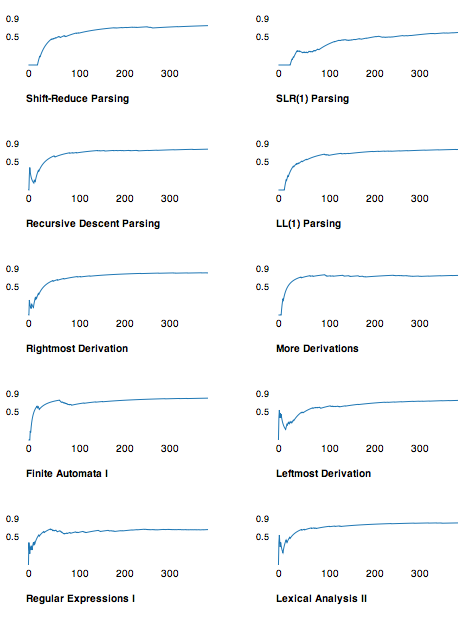
\includegraphics[width=1\columnwidth]{proofcache}
\caption{We graph cache hit rates against time for all assignments. The x-axis measures the total number of interactions with DeduceIt. The y-axis measures cache hit rates as a percentage.}
\label{fig:proofcache}
\end{figure}

\subsection{Performance Impact of the Cache}

In the final experiment, we measure the impact of DeduceIt's proof cache on overall system efficiency. As we have discussed, the time cost differential between a call to the Prover API and a proof cache lookup is high --- $900ms$ vs $4300ms$. This suggests that as long as the hit rate of the proof cache is also relatively high, the cache will provide the system with enormous time savings. 

In figure \ref{fig:proofcache}, we show the cache hit rate plotted against time. Although there are some differences in these plots, in each case the proof cache rises to a high hit rate very quickly. In every case, by the $Xth$ student interaction, the cache has reached a hit rate of $85\%$. From this, we can safely accept a $15\%$ hit rate as a lower bound. To measure the overall gain in efficiency from the cache we can compute:
$$Cache: 4000*0.15 + 1000 = 1600ms$$
This is meant to be a conservative estimate; the system latency we measure empirically is $900ms$. And when evaluated against a system without the cache---at $4000ms$ per interaction---this represents a cost savings of $60\%$.

High cache hit rates suggest that students tend to follow similar paths through their derivations. In table \ref{tab:table2} we show the number of unique assignment derivations compared against the overall cache hit rate for each assignment. [Fixme: acutally do this.]

\subsection{New Possibilities for Analysis}

Out of the 11 DeduceIt assignments, we look more closely at \textit{Regular Expressions I}, \textit{Leftmost Derivation}, and \textit{LL(1) Parsing} to show the new kinds of analyses which DeduceIt enables: \textit{Regular Expressions I} asks students to prove equivalence between two regular expression, \textit{Leftmost Derivation} asks students to perform a leftmost derivation using a provided grammar, and \textit{LL(1) Parsing} asks students to derive a string using a the provided LL(1) parsing table. We chose these assignments as representative examples which become progressively more difficult.

[Fixme: We never discussed this, but it seems like a good idea. What are some cool ideas/applications for assignment data?]

\section{Conclusions}

Fixme: real conclusion

\balance

% If you want to use smaller typesetting for the reference list,
% uncomment the following line:
% \small
\bibliographystyle{acm-sigchi}
\bibliography{actual}
\end{document}
